\documentclass[11pt, a4paper]{article}

% Idioma y codificación
\usepackage[utf8]{inputenc}
\usepackage[spanish, es-tabla]{babel}

% Ajuste de márgenes de página
\usepackage{geometry}
\geometry{
  top=2.5cm,
  bottom=2.5cm,
  left=2.5cm,
  right=2.5cm
}

% Paquetes complementarios indispensables
\usepackage{graphicx}
\usepackage{hyperref}
\usepackage{listings}
\usepackage{xcolor}
\usepackage{amsmath}
\usepackage{amssymb}
\usepackage{caption}

% Configuración del paquete hyperref para enlaces interactivos
\hypersetup{
    colorlinks=true,
    linkcolor=blue,
    filecolor=magenta,      
    urlcolor=blue,
    pdftitle={Actividad 9 - Programación Dinámica},
    pdfpagemode=UseNone,
}

% Paleta de colores para el código Java
\definecolor{codegreen}{rgb}{0,0.6,0}
\definecolor{codegray}{rgb}{0.5,0.5,0.5}
\definecolor{codepurple}{rgb}{0.58,0,0.82}
\definecolor{codeblue}{rgb}{0.0,0.2,0.6}
\definecolor{backcolour}{rgb}{0.97,0.98,0.99}

% Estilo de listings profesional para Java
\lstdefinestyle{javastyle}{
    backgroundcolor=\color{backcolour},   
    commentstyle=\color{codegreen}\itshape,
    keywordstyle=\color{codeblue}\bfseries,
    numberstyle=\tiny\color{codegray},
    stringstyle=\color{codepurple},
    basicstyle=\ttfamily\scriptsize\color{black},
    breakatwhitespace=false,         
    breaklines=true,                 
    captionpos=b,                    
    keepspaces=true,                 
    numbers=left,                    
    numbersep=8pt,                  
    showspaces=false,                
    showstringspaces=false,
    showtabs=false,                  
    tabsize=4,
    language=Java,
    extendedchars=true,
    % Mapeo de caracteres UTF-8 en español para evitar errores en listings
    literate={á}{{\'a}}1 {é}{{\'e}}1 {í}{{\'i}}1 {ó}{{\'o}}1 {ú}{{\'u}}1 {ñ}{{\~n}}1 {Á}{{\'A}}1 {É}{{\'E}}1 {Í}{{\'I}}1 {Ó}{{\'O}}1 {Ú}{{\'U}}1 {Ñ}{{\~N}}1
}
\lstset{style=javastyle}

% Datos del Documento
\title{
    \vspace{-1.5cm}
    \textbf{\Large Actividad 9: Programación Dinámica} \\
    \large Curso: Análisis y Diseño de Algoritmos
}
\author{
    \textbf{Repositorio GitHub:} \href{https://github.com/ZapanaDiego/Analisis-y-Disenio-de-Algoritmos/tree/main/ProgramacionDinamicaActividad09}{\texttt{Enlace al Repositorio Aquí}}
}
\date{} % Se deja vacío para eliminar la fecha

\begin{document}

\maketitle

\section{Problema de las Escaleras}

\subsection{Explicación del Algoritmo}
El problema requiere calcular las formas diferentes de subir una escalera de $N$ escalones avanzando de a $1$ o $2$ pasos. Al tener subestructura óptima, para llegar al escalón $i$, obligatoriamente se tuvo que dar un paso desde el escalón $i-1$ o desde el escalón $i-2$. Por tanto, las formas de llegar a $i$ son la suma de las formas de llegar a sus dos escalones predecesores (similar a la sucesión de Fibonacci).

\subsection{Estado de la Programación Dinámica}
Se utiliza un arreglo unidimensional $dp$, donde:
\[
dp[i] = \text{Número de formas distintas de llegar al escalón } i.
\]

\subsection{Relación de Recurrencia}
Para cualquier escalón $i \ge 2$:
\[
dp[i] = dp[i-1] + dp[i-2]
\]

\subsection{Casos Base}
Los casos base corresponden a situaciones donde no es necesario realizar saltos o la escalera es muy corta:
\begin{itemize}
    \item $dp[0] = 1$: Representa el estado inicial (estar en el suelo). Hay una única forma de estar ahí: no dar ningún paso.
    \item $dp[1] = 1$: Solo hay una forma de llegar al primer escalón: dando un paso de $1$ escalón desde el suelo.
\end{itemize}

\subsection{Análisis de Complejidad}
\begin{itemize}
    \item \textbf{Complejidad Temporal $\mathcal{O}(N)$:} Se ejecuta un ciclo lineal único que va desde el escalón $2$ hasta el escalón $N$. En cada iteración se realiza una suma básica en tiempo constante $\mathcal{O}(1)$. Por lo tanto, el tiempo de ejecución crece de manera directamente proporcional al número de escalones $N$.
    \item \textbf{Complejidad Espacial $\mathcal{O}(N)$:} El algoritmo requiere instanciar una tabla (arreglo unidimensional) de tamaño $N+1$ para almacenar los resultados del estado DP en cada posición intermedia. Esto implica un uso de memoria que escala linealmente en función de $N$.
\end{itemize}

\subsection{Código Fuente}
A continuación se muestra la implementación completa del algoritmo en Java, incluyendo el menú interactivo para el usuario:

\lstinputlisting[caption={Implementación en Java del Problema de las Escaleras}, label={lst:escaleras}]{codigo/Escaleras.java}

\subsection{Evidencias de Ejecución}
La implementación se validó ejecutando casos de prueba y permitiendo una entrada interactiva. A continuación se incluye la captura de pantalla con los resultados arrojados por consola.

\begin{figure}[htbp]
    \centering
    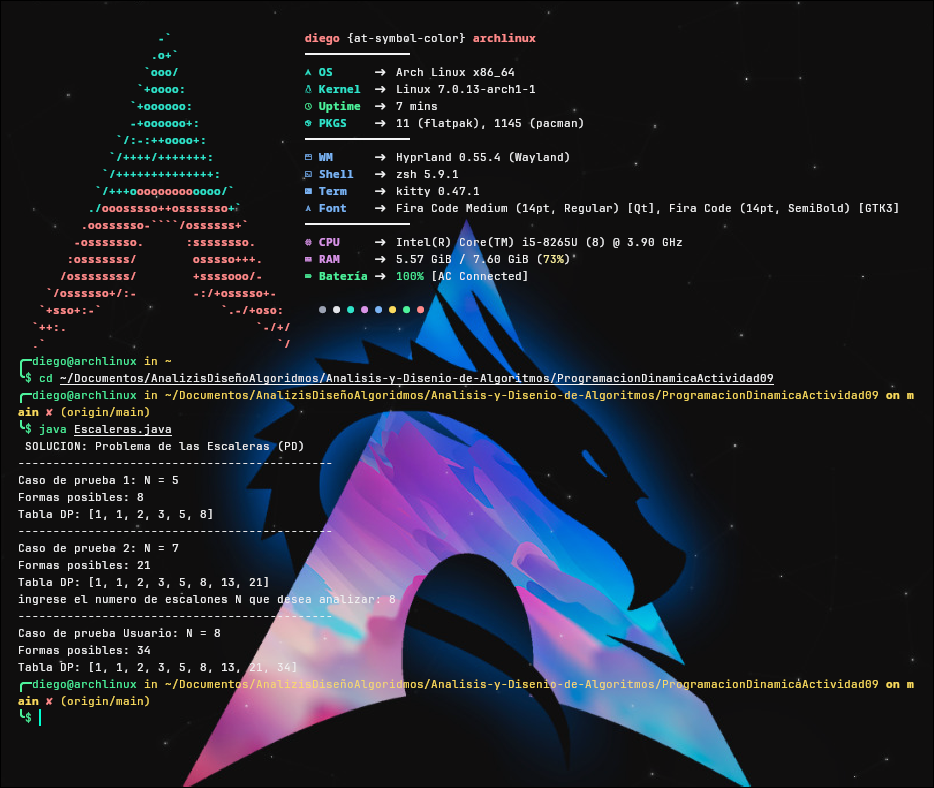
\includegraphics[width=0.8\textwidth]{img/captura_escaleras.png}
    \caption{Captura de pantalla de la ejecución mostrando la tabla DP [1, 1, 2, 3, 5, 8] para N=5.}
    \label{fig:captura_escaleras}
\end{figure}

\newpage

\section{Problema del Cambio Mínimo de Monedas}

\subsection{Explicación del Algoritmo}
El objetivo es encontrar la cantidad mínima de monedas necesarias para sumar una cantidad $C$, disponiendo de un conjunto de $M$ denominaciones de monedas. A diferencia del enfoque ávido (\textit{greedy}), el cual puede fallar o retornar soluciones subóptimas para sistemas de monedas no canónicos, la Programación Dinámica garantiza la obtención de la solución óptima global.

Utilizamos un enfoque Bottom-Up de abajo hacia arriba. Construimos las soluciones óptimas para todos los montos intermedios $i$ desde $1$ hasta la cantidad objetivo $C$. Para cada monto $i$, iteramos a través del conjunto de denominaciones y evaluamos si tomar una moneda de valor $moneda$ nos da una solución mejor que la registrada previamente. Además, para la reconstrucción del camino óptimo, se registra qué denominación de moneda fue elegida para cada monto en una tabla auxiliar.

\subsection{Estado de la Programación Dinámica}
Definimos el estado de la programación dinámica en una tabla $dp$ de tamaño $C+1$, donde:
\[
dp[i] = \text{Cantidad mínima de monedas necesarias para formar el monto } i.
\]

\subsection{Relación de Recurrencia}
Para cada monto intermedio $i$ (desde $1$ hasta $C$), la relación de actualización es:
\[
dp[i] = \min_{moneda \in \text{Monedas}, \, moneda \le i} \left( dp[i], \, dp[i - moneda] + 1 \right)
\]

\subsection{Casos Base}
Los límites iniciales se establecen de la siguiente manera:
\begin{itemize}
    \item $dp[0] = 0$: Se requieren exactamente cero monedas para representar un monto de valor $0$.
    \item $dp[i] = \infty$ para todo $i > 0$: Inicialmente asumimos que todos los montos mayores a $0$ son inaccesibles, representados con un valor infinito práctico (\texttt{Integer.MAX\_VALUE} en Java, controlando el desbordamiento de enteros al sumar).
\end{itemize}

\subsection{Análisis de Complejidad}
\begin{itemize}
    \item \textbf{Complejidad Temporal $\mathcal{O}(M \cdot C)$:} El algoritmo cuenta con dos ciclos anidados. El ciclo externo recorre todos los montos intermedios $i$ de $1$ a $C$, y el ciclo interno evalúa las $M$ denominaciones de monedas disponibles. Dado que se realizan operaciones aritméticas y comparaciones elementales $\mathcal{O}(1)$ dentro de los ciclos, el tiempo total es proporcional a la multiplicación de ambas variables.
    \item \textbf{Complejidad Espacial $\mathcal{O}(C)$:} Se utilizan dos arreglos de tamaño $C+1$: el primero (\texttt{dp}) almacena los montos mínimos y el segundo (\texttt{monedaUsada}) guarda el valor de la moneda elegida para la posterior reconstrucción de la combinación. El espacio total es lineal en relación al monto $C$.
\end{itemize}

\subsection{Código Fuente}
A continuación se presenta la implementación del algoritmo de Cambio de Monedas en Java, la cual incorpora la lógica de reconstrucción de la combinación óptima de monedas empleada:

\lstinputlisting[caption={Implementación en Java del Cambio Mínimo de Monedas}, label={lst:monedas}]{codigo/CambioMonedas.java}

\subsection{Evidencias de Ejecución}
Se ejecutaron pruebas unitarias automatizadas y pruebas personalizadas mediante el scanner. La captura de pantalla en la figura \ref{fig:captura_monedas} valida el comportamiento correcto y la visualización de la traza de monedas.

\begin{figure}[htbp]
    \centering
    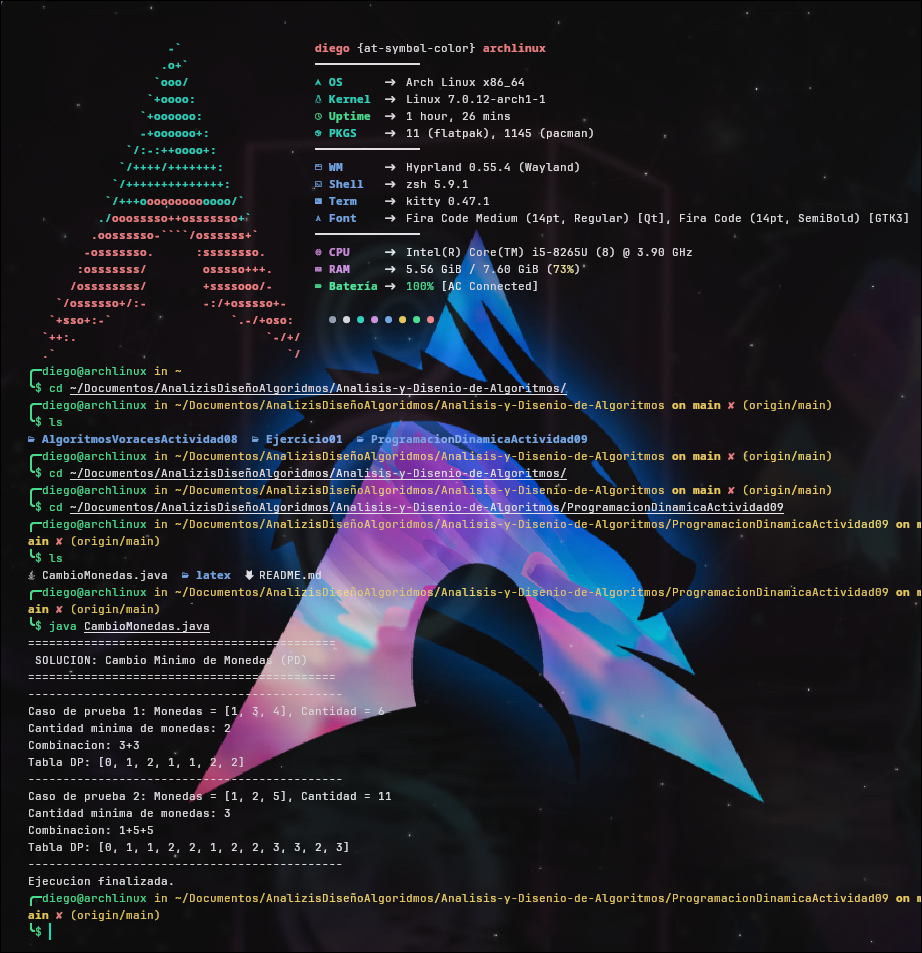
\includegraphics[width=0.8\textwidth]{img/captura_monedas.png}
    \caption{Captura de pantalla de la ejecución que muestra la solución correcta y la trazabilidad (combinación de monedas empleadas).}
    \label{fig:captura_monedas}
\end{figure}

\end{document}